\section{Анализ электронных писем Хиллари Клинтон}

\subsection{Количества слов}

\begin{itemize}

\item Гистограмма распределения количества слов каждой длины: 

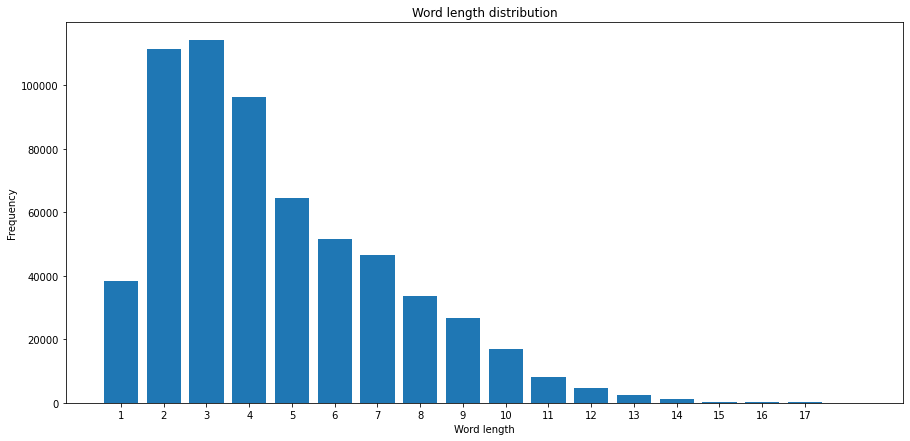
\includegraphics[scale=0.5]{pics/word_lengths.png}

Гистограмма выглядит вполне естественным образом, много коротких слов (например, местоимений, предлогов).

\item Гистограмма распределения длин (в количестве слов) писем:

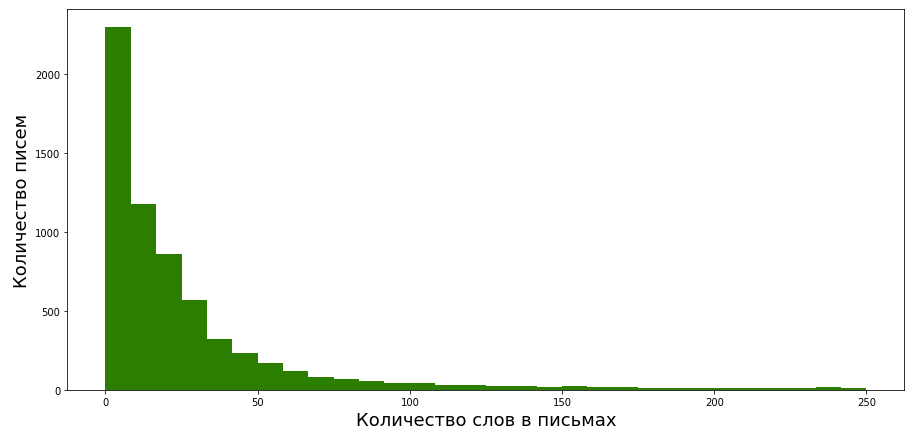
\includegraphics[scale=0.5]{pics/email_lengths.png}

Гистограмма соответствует интуитивным ожиданиям -- более длинные письма пишутся реже. 
\end{itemize}

\subsection{Время отправки писем}

\begin{itemize}

\item Количество отправленных писем по годам:

$ $

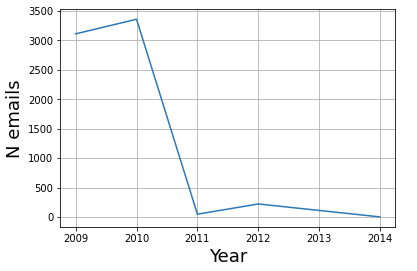
\includegraphics[scale=0.8]{pics/year.png}

На графике можно заметить странную аномалию с нулем писем в 2011 году. Вероятнее всего, это связано с особенностями набора данных. 

\item Количество отправленных писем по дням недели:

$ $

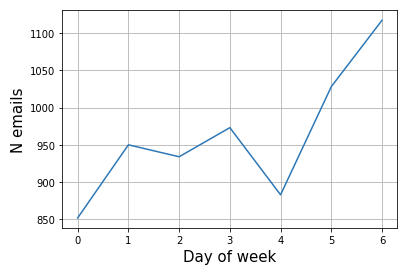
\includegraphics[scale=0.8]{pics/week.png}

График выглядит слегка неестественно (в отличие от \textit{Enron}). Можно попытаться интерпретировать это как особенности одного отдельного человека, занимающего специфичным видом деятельности.
\end{itemize}
